\chapter{Kubernetes}
Als Resultat jahrelanger Erfahrung die Google im Bau von Container-Anwendungen, sowie deren Betrieb in Clustern gemacht hat, bildet Kubernetes eines der wohl am häufigsten genutzten Managementtools für Container innerhalb eines Docker Clusters.\\
Von Beginn an dazu entwickelt Deployment und Skalierung von Containern zu automatisieren, hat sich das am 07. Juni 2014 als Open Source Plattform erstmals vorgestellte Kubernetes neben Apaches Mesos oder Hadoop YARN etabliert und wird im folgenden Kapitel vorgestellt.\\
Dabei werden verschiedene Aspekte wie Architektur, Skalierung oder Persistenz betrachtet und ein Vergleich zu Docker Swarm als Alternative gezogen.


\section{Architektur}
\begin{figure}
	\centering
	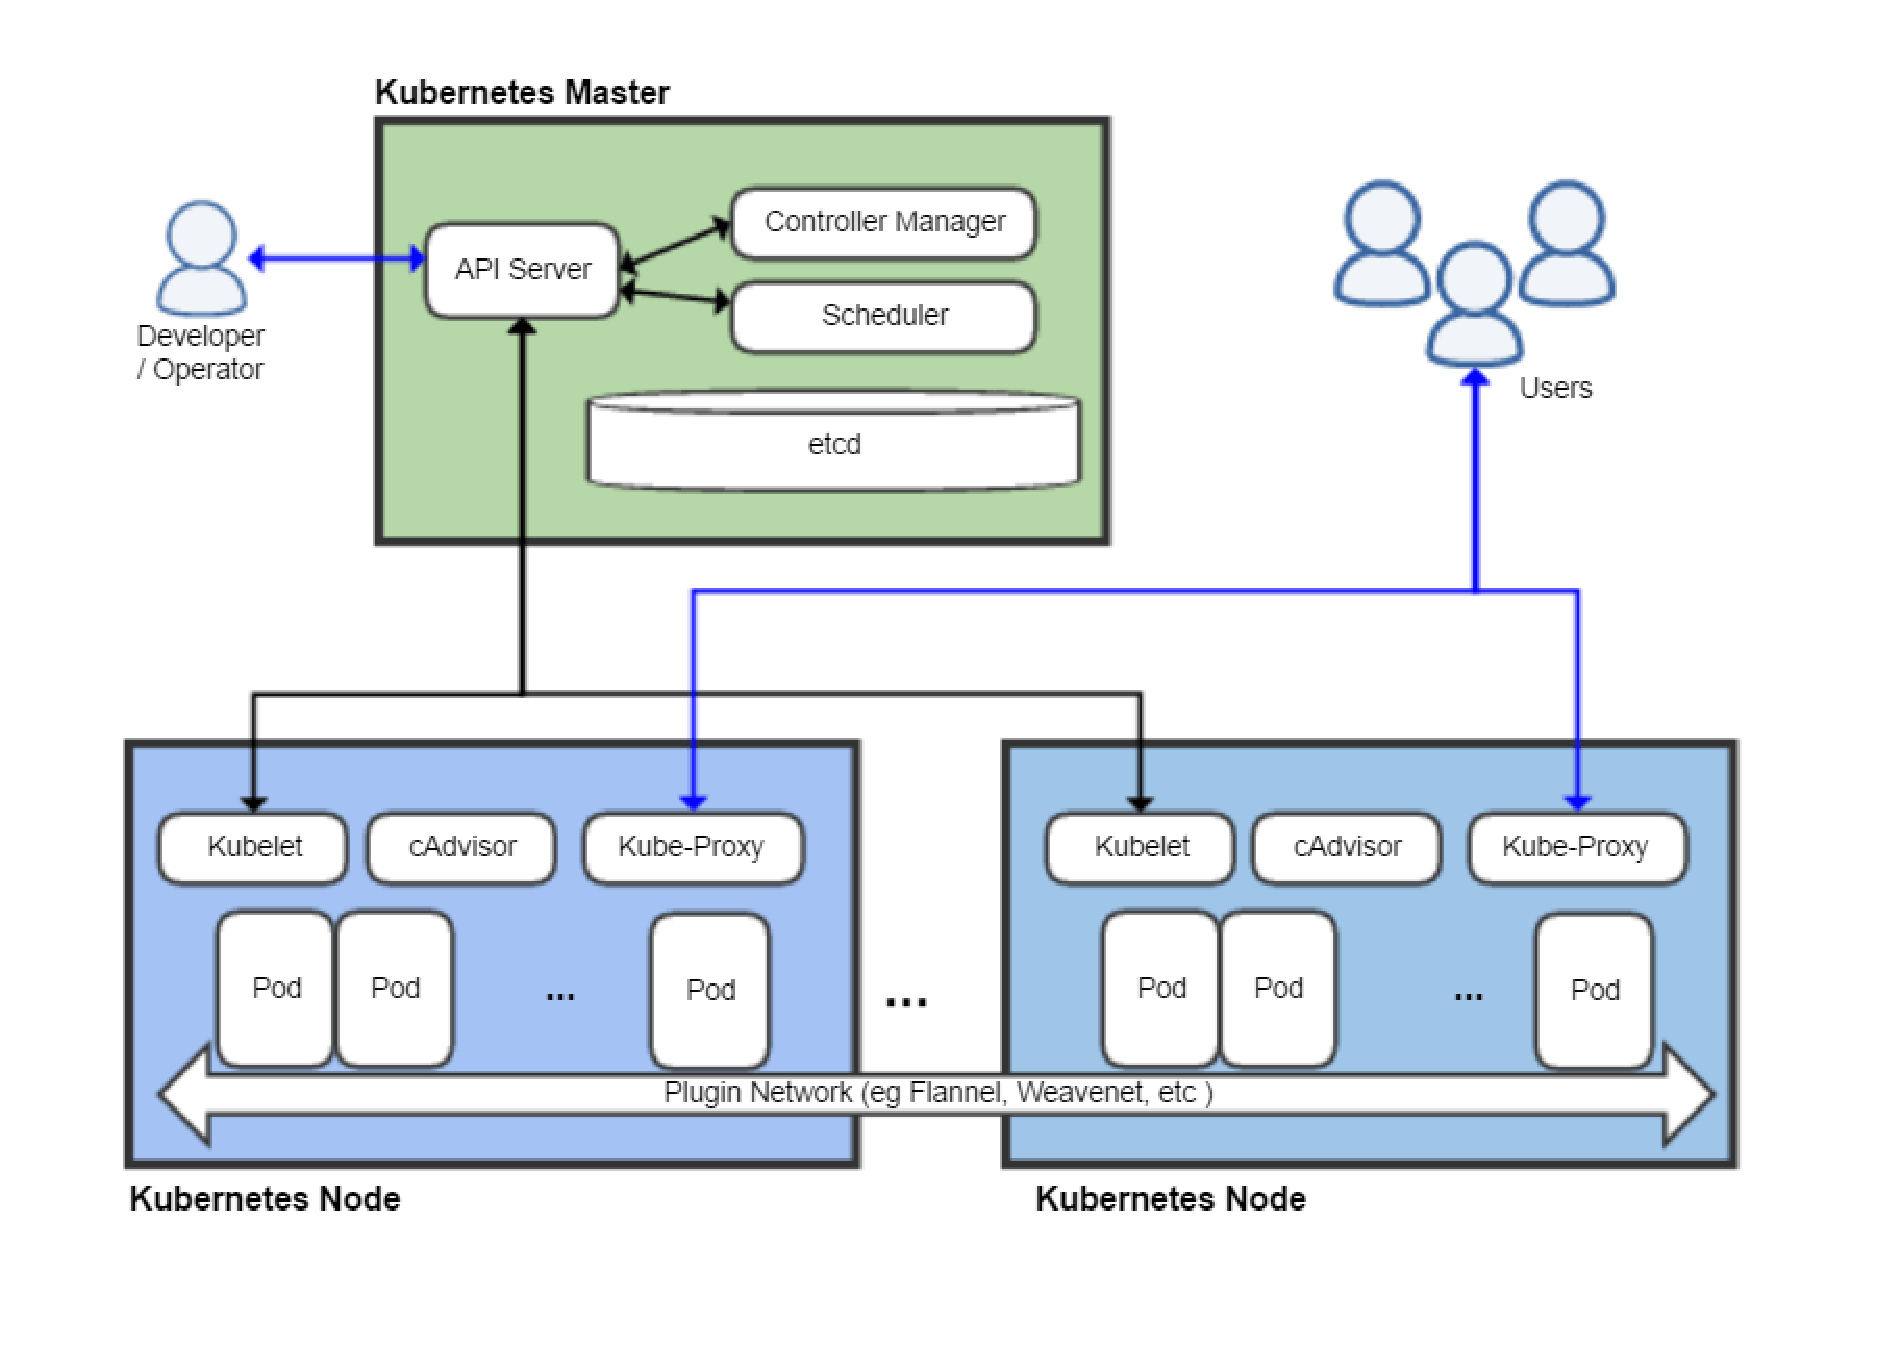
\includegraphics[width=0.9\linewidth]{figures/kubernetes-architecture}
	\caption[Kubernetes Architekture]{Kubernetes Architektur im Cluster}
	\label{fig:kubernetes-architecture}
\end{figure}
Die Architektur von Kubernetes entspricht dem Master-Slave Prinzip wie Abbildung \ref{fig:kubernetes-architecture} schematisch zeigt. Dabei steuert der Master die Nodes auf denen die Docker Container laufen.\\
Der Kubernetes Master ist besteht im wesentlichen aus drei Prozessen die auf einem einzelnen Knoten des Clusters laufen. Dieser wird häufig auch Master Node genannt und besteht aus folgenden Komponenten:
\begin{itemize}
	\item API Server - zentrale Komponente, die via REST Schnittstelle allen anderen Komponenten Informationen bereitstellt.
	\item Scheduler - überwacht die Last der einzelnen Nodes und entscheidet abhängig von verfügbaren Ressourcen auf welcher Node weitere Pods gestartet werden.
	\item Controller Manager - enthält alle Kontrollmechanismen und kommuniziert mit dem API Server um den aktuellen Zustands des Clusters zu überwachen und diesen in den gewünschten Zustand zu überführen.
	\item etcd - leichtgewichtige Key-Value Datenbank zur Speicherung der Cluster Konfiguration. Diese Enthält den Gesamtzustand des Clusters und wird vom API Server genutzt.
\end{itemize}\newpage
Die übrigen Nodes, ehemals Minions genannt, bilden einzelne Server auf denen Container gestartet werden können. Jeder Node stellt eine Container Laufzeitumgebung zur Verfügung und besteht aus folgenden Komponenten:
\begin{itemize}
	\item Kubelet - zentrale Komponente einer Node und überwacht als solche den aktuellen Status der Node und meldet diese an den Controller Manager. Dieser gibt dann Anweisung zum Starten oder Stoppen von Containern. Fällt ein Container aus wird er vom Kubelet auf der gleichen Node neu gestartet. Fällt die komplette Node aus, wird dies vom Master aufgrund ausbleibender Statusmeldung erkannt und die Pods werden auf anderen Nodes neu gestartet.
	\item Kube-Proxy - implementiert Netzwerk Proxy und Load Balancer. Routet abhängig von IP Adresse und Port eingehenden Netzwerkverkehr an die entsprechenden Container.
	\item cAdvisor - ist im Kubelet integriert und zeichnet die Ressourcen eines Containers auf, um diese anderen Monitoringlösungen zur Auswertung von Metriken bereitzustellen.
\end{itemize}
\newpage
\section{Skalierung}
Eines der nativen Features von Kubernetes ist die automatische horizontale Skalierung.\\Verantwortlich dafür ist ein Teil des Controller Managers, der "Horizontal Pod Autoscaler".
Dieser bekommt über eine Konfiguration mitgeteilt, wie oft er die Auslastung welcher Ressourcen abfragen soll und wie er diese zu interpretieren hat.\\
Die Metriken werden vom Controller Manager über eine eigene API, speziell für die Auslastung von Ressourcen gewonnen. Dabei können nicht nur Informationen pro Pod abgefragt, sondern auch benutzerdefinierte Messwerte ausgelesen werden.\\
Grundsätzlich können die Messwerte entweder als Auslastungs-Wert oder Rohwert interpretiert werden.\\
Im ersteren Fall berechnet der Controller zuerst den Nutzungswert als Prozentsatz der entsprechenden Nachfrage nach Ressourcen für die Container in jedem Pod.
Ist der Roh-Wert konfiguriert so entfällt der erste Schritt und der Messwert wird direkt übernommen.\\
Anschließend berechnet der Controller ausgehend vom Ergebnis aus erstem Schritt oder dem Rohwert einen Mittelwert über alle zu skalierenden Pods welcher dann als Verhältnis dient, wie viele neue Pods repliziert werden müssen.
\\\\
Ebenfalls konfigurierbar sind die Schwellenwerte für die Verzögerungen beim Hoch- und Runterskalieren. Diese müssen jedoch mit bedacht gewählt werden, ist die Verzögerung zu hoch eingestellt reagiert der Autoscaler nicht schnell genug auf erhöhte Last. Umgekehrt kann es bei zu niedriger Verzögerung und sich zu schnell ändernden Lasten zu unnötigem Overhead und Ressourcenverbrauch aufgrund ständig neu erzeugter Container kommen.
\section{Persistenz}
Eines der grundsätzlichen Probleme von Container-Anwendungen ist die Persistenz von Daten. Das gängige Vorgehen Daten in einem Container zur Verfügung zu stellen sind Volumes. Das Problem von Volumes ist ihre Flüchtigkeit.
Stürzt ein Container ab, so wird er vom Kubelet neu gestartet doch die Daten sind dann nicht mehr verfügbar da der Container in seinem Initialzustand gestartet wird.\\
Laufen Container-Anwendungen in einem Cluster, teilen diese häufig Ressourcen untereinander, bzw. greifen gemeinsam darauf zu.\\
Doch wie stellt man Ressourcen für Anwendungen bereit, die auf verschiedenen Servern laufen?
Kubernetes bietet hierfür eine Lösung in Form von Persistent Volumes.\\
Diese können als Ressource innerhalb des Clusters, ähnlich einer Node betrachtet werden und werden vom Administrator bereitgestellt wird. Sie können von Containern wie Volumes genutzt werden, haben aber einen Lebenszyklus der unabhängig von den Pods ist die auf das persistente Volume zugreifen.
\newpage
\section{Service Discovery und Load Balancing}
Kubernetes Pods sind Eintagsfliegen. Sie werden vom Replication Controller erzeugt, gestartet, später gestoppt und gelöscht. Auch wenn jedem Pod eine eigene IP Adresse vergeben wird ändert sich diese dennoch je nach Verfügbarkeit. 
Dies führt zu folgendem Problem:\\
Wenn eine Gruppe Pods - Backend genannt - Funktionalität für eine andere Gruppe Pods - Frontend gennant - bereitstellt, wie finden die Frontend Pods die Backend Pods?\\
Hier kommen Services ins Spiel.\\\\
Ein Kubernetes Service ist eine abstrakte Definition einer Gruppe von Pods und Regeln, wie diese angesprochen werden können. Manchmal werden diese auch Micro-Service genannt.\\\\
\begin{minipage}{\linewidth}
\begin{lstlisting}[frame=single,caption=Kubernetes Service Definition, label=kubernetesServiceDefinition, language=Scala]
kind: Service
apiVersion: v1
metadata:
  name: my-service
  spec:
    selector:
      app: MyApp
    ports:
    - protocol: TCP
      port: 80
      targetPort: 9376
\end{lstlisting}
\end{minipage}
Beispiel \ref{kubernetesServiceDefinition} zeigt eine Service Definition mit der ein Service Objekt namens ``my-service`` erzeugt wird, das in jedem zugehörigen Pod mit dem Label ``app=MyApp`` den TCP Port 9376 verfügbar macht.
In einem Service Objekt kann ein eingehendes Port auf ein beliebiges Port am Pod gemappt werden.\\\\
Interessanter ist die Möglichkeit, statt einer Port Nummer einen String mit einer Referenz auf ein Port angeben zu können. Dies ergmöglicht es, die tatsächliche Port Nummer welche dieser Referenz zugewiesen wird, in jedem Pod innerhalb der Gruppe unterschiedlich zu konfigurieren, was das Deployment und die Weiterentwicklung von Services sehr flexibel macht. So können etwa in der nächsten Version des Backends die offenen Ports der Pods geändert werden während das Backend dennoch für die Clients erreichbar bleibt.
\\\\
Kubernetes unterstützt grundsätzlich zwei Modi zur Service Discovery - Umgebungsvariablen und DNS.\\
Wenn ein Pod innerhalb einer Node gestartet wird fügt das Kubelet automatisch eine Reihe von Umgebungsvariablen für jeden aktiven Service an. So werden zum Beispiel für den Service ``redis-master``, der unter der Cluster IP Adresse 10.0.0.11 und TCP Port 6379 erreichbar ist, die in Beispiel \ref{kubernetesEnvVariables} gezeigten Umbgebungsvariablen angelegt.\\
\begin{minipage}{\linewidth}
	\begin{lstlisting}[frame=single,caption=Umgebungsvariablen für Service ``redis-master``, label=kubernetesEnvVariables, language=bash]
REDIS_MASTER_SERVICE_HOST=10.0.0.11
REDIS_MASTER_SERVICE_PORT=6379
REDIS_MASTER_PORT=tcp://10.0.0.11:6379
REDIS_MASTER_PORT_6379_TCP=tcp://10.0.0.11:6379
REDIS_MASTER_PORT_6379_TCP_PROTO=tcp
REDIS_MASTER_PORT_6379_TCP_PORT=6379
REDIS_MASTER_PORT_6379_TCP_ADDR=10.0.0.11
	\end{lstlisting}
\end{minipage}\\\\
Dies impliziert eine gewisse Reihenfolge. Jeder Service den ein Pod nutzen soll muss entsprechend vor dem Pod erzeugt werden, da ansonsten die Umgebungsvariablen nicht angelegt werden können.\\\\
Service Discovery über DNS unterliegt dieser Einschränkung dagegen nicht.\\
Ein DNS Server kann als optionale Komponente dem Cluster hinzugefügt werden. Dieser fragt den API Server nach neuen Services ab und legt für jeden eine Reihe DNS Einträge an.\\\\
Nehmen wir erneut den ``my-service`` als Beispiel und nehmen an, dass dieser im Namespace ``my-ns`` erreichbar ist, so legt der DNS Server einen Eintrag für ``my-service.my-ns`` an. 
Pods, die im ``my-ns`` Namespace liegen können den Service erreichen indem sie den Namen ``my-service`` auflösen.\\
Pods die in anderen Namespaces liegen müssen entsprechend den Namen ``my-service.my-ns`` auflösen. In beiden Fällen wird als Resultat die IP Adresse innerhalb des Clusters geliefert.\\
Kubernetes unterstützt ebenfalls DNS Einträge für Service Definitionen mit benamten Ports. Enthält beispielsweise die Definition des ``my-service.my-ns`` ein mit ``http`` referenziertes TCP Port, so kann über eine DNS Namensauflösung nach ``\_http.\_tcp.my-service.my-ns`` die entsprechende Port Nummer herausgefunden werden.\\\\
In manchen Fällen ist es nötig Services innerhalb des Clusters auch von außerhalb erreichbar zu machen. Kubernetes bietet hierfür verschiedene Möglichkeiten von Service Typen an. An dieser Stelle soll im speziellen nur auf den Typ Load Balancer eingegangen werden.\\
Abhängig vom Cloud Hoster wird für einen Service, der mit Typ Loadbalancer definiert ist, automatisch ein externer Loadbalancer vorgeschaltet. Dieser Vorgang geschieht asynchron und die entsprechende Statusinformation wird im ``status.loadbalancer`` Feld des jeweiligen Service hinterlegt. Code Beispiel \ref{kubernetesLoadbalancerDefinition} zeigt eine mögliche Servicedefinition.\\
\begin{minipage}{\linewidth}
	\begin{lstlisting}[frame=single,caption=Kubernetes Service mit Loadbalancer Definition, label=kubernetesLoadbalancerDefinition, language=Scala]
kind: Service
apiVersion: v1
metadata:
  name: my-service
spec:
  selector:
    app: MyApp
  ports:
  - protocol: TCP
    port: 80
    targetPort: 9376
  clusterIP: 10.0.171.239
  loadBalancerIP: 78.11.24.19
  type: LoadBalancer
status:
  loadBalancer:
    ingress:
    - ip: 146.148.47.155
	\end{lstlisting}
\end{minipage}\\
Eingehender Netzwerkverkehr vom externen Loadbalancer wird dann an die entsprechenden Pods geroutet, wie genau dies jedoch geschieht hängt vom jeweiligen Cloud Hoster ab.\\\\
In gemischten Umgebungen kann es manchmal nötig sein auch Verkehr innerhalb des Clusters routen zu lassen. Dazu wären zwei Services nötig die sowohl intern als auch extern eingehenden Netzwerkverkehr zu den gwünschten Endpunkten routen können. Dies kann erreicht werden, indem in der Service Definition spezielle Annotations mit dem Hinweis auf einen internen Load Balancer hinterlegt werden.\\
\section{Batch Exectution}
TODO
\section{Kubernetes vs Docker Swarm}
Die derzeit am häufigsten genutzten Tools zum Cluster Management bilden Kubernetes und Docker Swarm weshalb an dieser Stelle noch ein kurzer Vergleich der beiden gezogen werden soll.\\
Der wohl größte Vorteil von Docker Swarm ist wohl das native Clustering von Docker Containern. Außerdem nutzt Swarm die gleiche API wie Docker, sodass Nutzer die gleichen Tools die sie mit Docker nutzen auch in Docker Swarm nutzen können ohne einen separaten Befehlssatz lernen zu müssen. Dies ist gleichermaßen auch ein Nachteil, da Tools die von Docker selbst nicht unterstützt werden auch in Docker Swarm nicht genutzt werden können. Außerdem bot Docker Swarm in seinen Anfängen keinerlei Möglichkeit für Persistenz.\\\\
Kubernetes dagegen wurde losgelöst von Docker entwickelt und bietet daher einiges an Flexibilität bei der Wahl von Tools. Diese Flexibilität wird aber mit einem gewissen Preis gewonnen. Während persistente und geteilte Volumes, Loadbalancer oder Service Discovery mitgeliefert werden, können diese nicht über die native Docker API genutzte werden. Auch müssen sämtliche Container und Service Definitionen die mit Docker, bzw. Docker Compose geschrieben wurden von Grund auf neu erstellt werden da Kubernetes andere YAML Definitionen als Docker nutzt.\\
Auch wenn Kubernetes einige Vorteile gegenüber Docker Swarm bietet, bringen Einstieg und Setup einiges an Overhead mit. Währenddessen hat Docker Swarm feature-technisch durchaus aufholen können und bietet einen annährenden Funktionumfang der ohne große Umstellung genutzt werden kann.